% Evaluation de la méthode de la completion/revision des PH
\section{Evaluation}
\label{sec:evaluation}
\subsection{Application: Circadian clock}

\begin{figure}
\begin{center}
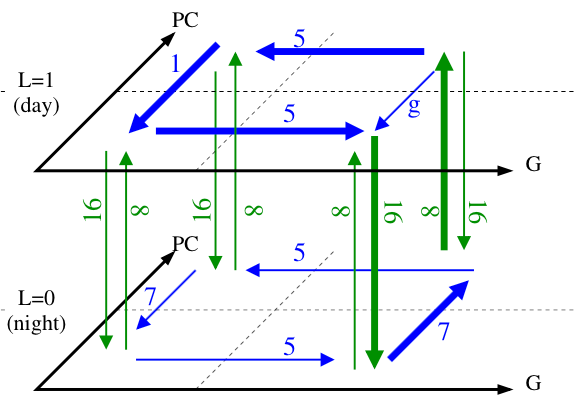
\includegraphics[width=0.4\linewidth]{images/circadianClock-summer.png}
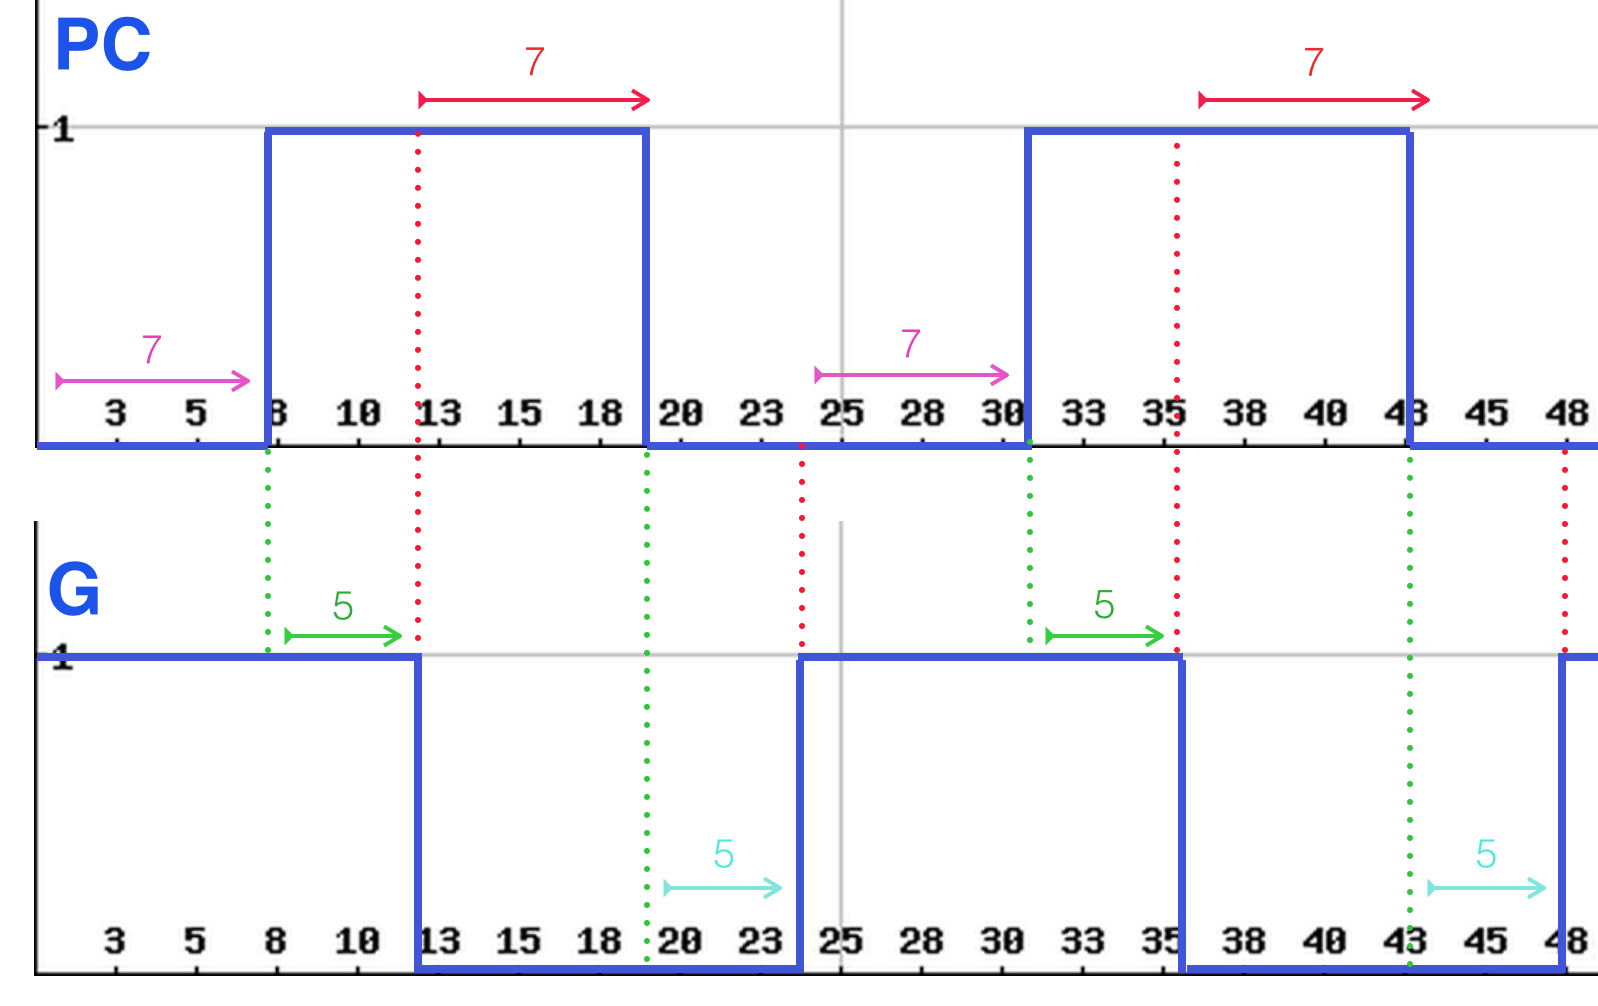
\includegraphics[width=0.4\linewidth]{images/circadianClock-Courb.png}
\end{center}
\caption{The qualitative model of the mammalian circadian cycle during during the summer from \cite{comet2010formal}. Discretization of the observed data set of circadian clock components during the night (L=0).}
\end{figure}

\begin{figure}
% TODO: revoir les actions du PH et d'ASP il faut qu'ils soient cohérents

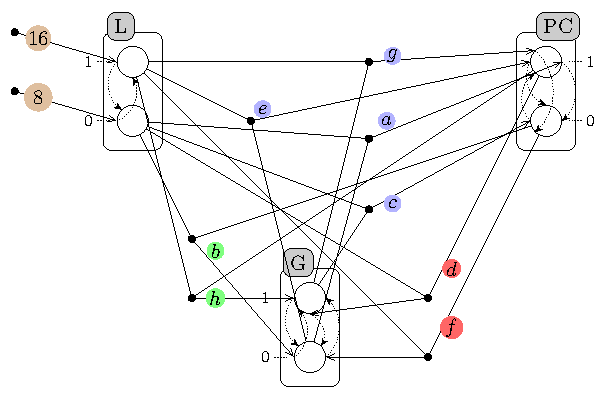
\includegraphics[width=0.4\linewidth]{images/circadianPH.pdf}
%
\hspace{1cm}
%
\begin{minipage}{0.5\linewidth}
	\textbf{Nodes:} \\
\texttt{{\footnotesize process("L",0..1).} }\\
\texttt{{\footnotesize process("PC",0..1).}}\\
\texttt{{\footnotesize process("G",0..1).} }\\

\textbf{Actions:} \\
\texttt{{\footnotesize action("G",1, "L",0, "PC",0,1, c).}} ~\\
\texttt{{\footnotesize action("G",0, "L",1, "PC",1,0, e).}} ~\\
\texttt{{\footnotesize action("PC",0, "L",1", "G",0,1, b).}} ~\\

\texttt{{\footnotesize action("G",0, "L",0", "PC",1,0, a).}} ~\\
\texttt{{\footnotesize action("PC",0, "L",0, "G",0,1, b).}} ~\\
\texttt{{\footnotesize action("PC",1, "L",0, "G",1,0, d).}} 
\end{minipage}
\end{figure}
%
\begin{figure}
\begin{center}
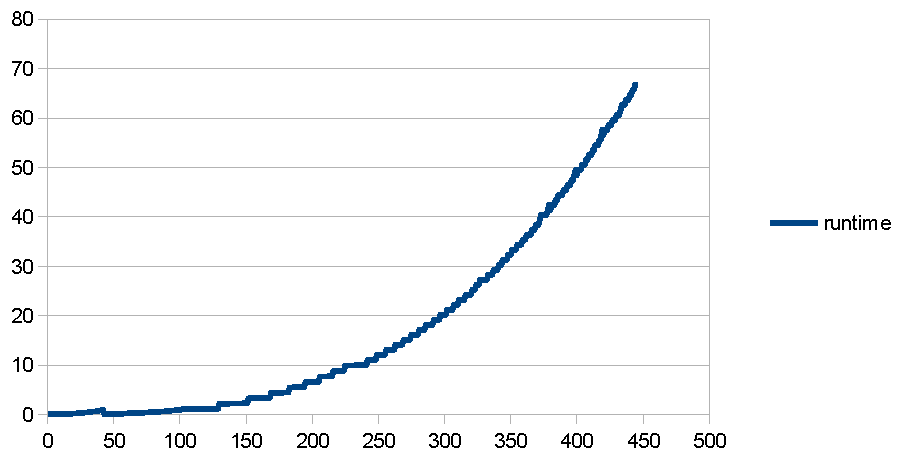
\includegraphics[width=0.6\linewidth]{images/run_time}
\end{center}
\caption{Run time of the application of  Algorithm \ref{alg:PHC_ap} on circadian clock chronograms varying the number of time steps.}
\end{figure}

\subsection{Benchmarks}
